% Preview source code

%% LyX 2.2.1 created this file.  For more info, see http://www.lyx.org/.
%% Do not edit unless you really know what you are doing.
\documentclass[12pt,english]{article}
\usepackage[T1]{fontenc}
\usepackage[latin9]{inputenc}
\usepackage[a4paper]{geometry}
\geometry{verbose,tmargin=0.5in,bmargin=0.5in,lmargin=0.5in,rmargin=0.5in,headheight=0.5cm,headsep=1.5cm,footskip=0.7cm}
\usepackage{fancyhdr}
\pagestyle{fancy}
\usepackage{color}
\usepackage{wrapfig}
\usepackage{textcomp}
\usepackage{amsmath}
\usepackage{graphicx}
\usepackage{setspace}
\usepackage[numbers]{natbib}
\onehalfspacing

\makeatletter
\@ifundefined{date}{}{\date{}}
%%%%%%%%%%%%%%%%%%%%%%%%%%%%%% User specified LaTeX commands.

%\usepackage{fullpage}

%%%%%%%%%%%%%%%%%%%%%%%%%%%%%% LyX specific LaTeX commands.
%% Because html converters don't know tabularnewline
\providecommand{\tabularnewline}{\\}

 % For LaTeX2e
%\usepackage{times}

\newcommand{\beginsupplement}{%
    \setcounter{table}{0}
    \renewcommand{\thetable}{S\arabic{table}}%
    \setcounter{figure}{0}
    \renewcommand{\thefigure}{S\arabic{figure}}%
 }

%\renewcommand{\vec}[1]{\mathbf{#1}}


%\global\long\def\fix{\marginpar{FIX}}
 %\global\long\def\new{\marginpar{NEW}}
 
 \DeclareMathOperator\erfc{erfc}
 
%\singlespacing





\usepackage[T1]{fontenc}
\usepackage{babel}
\usepackage[labelfont=bf]{caption}

\definecolor{red}{RGB}{136, 00, 34}

\makeatother

\usepackage{babel}
\begin{document}

\title{\vspace{-1.8cm}
\textbf{\textcolor{red}{\large{}Efficient replay memory through sensory adaptation\\ }}\vspace{-1cm}
}

%\author{{\normalsize{}Raymond Chua, David W Jia and Rui Ponte Costa}}

\maketitle
\begin{spacing}{1.1499999999999999}
\vspace{-0.8cm}
The cortex adapts quickly to repetitive stimuli. \textcolor{black}{Such adaptation suggests that dissimilar (or novel) experiences are more likely to be retained
in memory. In contrast, recent deep reinforcement learning models
rely on storing every single input into a hippocampal-like episodic
memory. Here, inspired by rapid forms of synaptic plasticity \textendash{} a key
neural basis of sensory adaptation \textendash{} we propose a reinforcement learning algorithm in which only dissimilar enough inputs are stored into the
replay memory. We show that our method leads to a more efficient memory
representation (reduced memory load), as similar inputs tend to be
discarded. In addition, a model in which less experiences are discarded
as the agent gradually learns to explore its environment performs similarly to standard replay memory methods.
This gradual change in adaptation is akin to the experimentally observed modifications of short-term
plasticity over development and
learning, and suggests an important role for this phenomenon in systems-level learning. Overall, our work shows how systems models of memory and learning can shed light on
the function of synaptic plasticity and sensory adaptation.}\vspace{-0.1cm}

\end{spacing}

\rule{0.9\columnwidth}{0.5pt}

\begin{spacing}{1.1499999999999999}
\vspace{0cm}

\end{spacing}

\begin{singlespace}
\begin{wrapfigure}[18]{R}{0.55\columnwidth}%
\begin{raggedleft}
\vspace{-0.7cm}
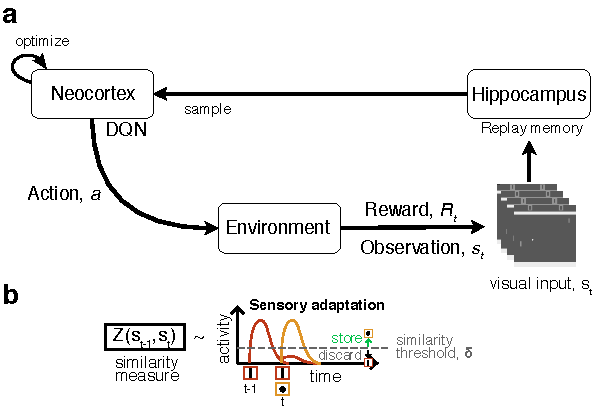
\includegraphics[clip,scale=1]{Figures/Fig1_Schematic_v3}
\par\end{raggedleft}
\vspace{-0cm}
\caption{\textit{Hippocampal-neocortical reinforcement learning architecture with sensory adaptation (modelled by similarity measure).}}
\vspace{-0.4cm}
\label{fig:1} \end{wrapfigure}

Both animals and artificial agents need to efficiently learn to explore their environments. As animals/agents sample the environment, the incoming state tends to be initially highly correlated in time, which leads to poor optimization of non-linear approximators, such as deep neural networks in the context of reinforcement learning. However, our brain seems to deal with this problem efficiently. Here, we focus mainly on the learning implications of temporal filtering mediated by sensory adaptation coupled with hippocampus-like experience replay (ER) (Fig.~1a).

Experience replay has enabled impressive results in deep RL (Mnih et al, 2015 Nature). On an abstract level, the \emph{experience replay} algorithm (Lin 1992 Machine Learning) can be interpreted as a simplified model of neocortical-hippocampal interactions during memory consolidation (Hassabis et al, 2017 Neuron). The hippocampal network allows for rapid learning of episodic memories, which are in turn gradually replayed to the neocortex for long-term memory storage -- systems memory consolidation (Ji et al, 2007 Nature). Following this view the neocortex implements a deep Q network (DQN, Fig.~1a), which is a multi-layered neural network that takes a state $s$ as input and outputs a vector of action-values. By using the parameters $d$ from DQN, with $d$ being the dimension of DQN, this allows us to approximate our function $Q(s,a; \boldsymbol{\theta})$. Hippocampal-like ER allows us to draw past experiences randomly (Fig.~1a), decorrelating experience examples and stabilising the algorithm during the learning phase.

%d = $\boldsymbol{\theta} \in \mathbb{R}^d$

\begin{figure}[t!]
    \centering
    \includegraphics[width=1\columnwidth]{Figures/multi_plots.pdf}
    \vspace*{-10mm}
    \caption{Filtered experience replay (FER; inspired by sensory adaptation) leads to a reduced replay memory load (middle and right) while achieving a similar performance (left) in Atari games when compared to standard experience replay (SER).}
    \label{fig:game_results}
\end{figure}

The key insight behind our model is that in many episodes an agent or an animal experiences tend be very similar/correlated. In RL terms, this means high similarity between consecutive states which leads to many similar experiences entering the replay memory (Fig.~1a). We drew inspiration from sensory adaptation to address this by comparing the input states using a similarity measure function as illustrated in Fig.~1b before the samples are added to the replay memory. Additionally, we consider two types of similarity threshold function, one that is constant and another in which the threshold decays over learning. Regarding the decay type, we consider two possible decay schemes, linear and exponential. The decay functions are defined as follows: $D_{\text{linear}}(t) = N_0 - \bigg(\frac{t}{f}\bigg)(N_0 - N_f)$ and $D_{\text{exp}}(t) = N_0 e^{-\lambda t}$, where $\lambda$ controls the decay rate, $t$ is the current step in environment, f is the decay constant, $N_0$ is the initial similarity value and $N_f$ is the final similarity value. In our experiments, we set $\lambda$ to 0.00001. The constant type has the same value throughout the learning phase, such that $N_0 = D_{\text{constant}}(t) = N_f$. In addition, we used the Normalised Root-Mean Square Error (NRMSE) function due to it being normalised and its ease/speed of computation. NRMSE is defined as $\mathrm{NRMSE}(Ix, Iy) = \frac{\sqrt{\mathrm{MSE}(Ix, Iy)}*\sqrt{n}}{\Vert  Ix \Vert }$ where $Ix$ and $Iy$ are greyscale images with $n$ pixels and MSE is the Mean Squared Error function. Our algorithm is a simple extension of DQN (Mnih et al, 2015 Nature).

% \begin{wrapfigure}[16]{R}{0.55\columnwidth}%
% \begin{raggedleft}
% \vspace{-0.5cm}
% %\includegraphics[clip,scale=0.55]{Figures/Fig3_v1}
% \par\end{raggedleft}
% \vspace{0.5cm}
% \caption{\textit{Network learns to solve a delayed contextual task.}}
% \vspace{-0.4cm}
% \label{fig:3} \end{wrapfigure}%

We tested our algorithm on four environments (Pong, Boxing, Enduro and Invaders) of the Arcade Learning Environment (Atari) (Bellemare et al, 2015 IJCAI). The training is initially performed over two million frames. We compared our algorithm against a baseline based on the original DQN algorithm (Mnih et al, 2015 Nature). We used Adam (Kingma et al, 2015 ICLR) as our optimizer with a mini-batch size of 32 and trained our model for two million frames, across five different seed values.

Inspired by changes in short-term plasticity over learning (Costa et al. 2015 eLife) and development (Reyes and Sackman 1999 JNeurosci), we tested scenarios in which the threshold $\delta$ varied with learning, using exponentially and linear decays (see above). Our results demonstrate that our method can yield more efficient experience replay (i.e. lower memory load, Fig.~2 middle and right) while retaining a comparable performance  (Fig.~2 left). This implies that our model provides a more efficient learning method compared to standard methods.

Finally, we are currently exploring 
a version of the model that automatically selects which inputs to discard using a simplified form of short-term plasticity at the synaptic level that is tuned during learning.

By combining abstract models of different brain areas and synaptic properties our work provides interesting insights into their interaction and suggests important roles when learning to explore complex environments. Moreover, it predicts that more correlated memories are stored in the hippocampal system as learning progresses, and that this is an important contributor to the exploration-exploitation trade off.

%\begin{wrapfigure}{r}{0.5\columnwidth}%
%\begin{raggedleft}
%\vspace{-1.3cm}
%\includegraphics[clip,width=0.25\columnwidth]{Figures/Fig1_v1}
%\par\end{raggedleft}
%\vspace{-0.7cm}
%\label{fig:net}
%\caption{\textit{Recurrent cortical microcircuit derived from objective function.}}
%\vspace{-0.4cm}
%\label{fig:framework} \end{wrapfigure}%


%\begin{wrapfigure}[18]{L}{0.55\columnwidth}%
%\begin{raggedleft}
%\vspace{-0.5cm}
%%\includegraphics[clip,scale=0.82]{Figures/Fig_2_v3}
%\par\end{raggedleft}
%\vspace{-0.25cm}
%\caption{\textit{StatLTSP explains slice experiments.}}
%\vspace{-0.5cm}
%\label{fig:results1} \end{wrapfigure}%



\end{singlespace}

\end{document}